% This is the Reed College LaTeX thesis template. Most of the work
% for the document class was done by Sam Noble (SN), as well as this
% template. Later comments etc. by Ben Salzberg (BTS). Additional
% restructuring and APA support by Jess Youngberg (JY).
% Your comments and suggestions are more than welcome; please email
% them to cus@reed.edu
%
% See http://web.reed.edu/cis/help/latex.html for help. There are a
% great bunch of help pages there, with notes on
% getting started, bibtex, etc. Go there and read it if you're not
% already familiar with LaTeX.
%
% Any line that starts with a percent symbol is a comment.
% They won't show up in the document, and are useful for notes
% to yourself and explaining commands.
% Commenting also removes a line from the document;
% very handy for troubleshooting problems. -BTS

% As far as I know, this follows the requirements laid out in
% the 2002-2003 Senior Handbook. Ask a librarian to check the
% document before binding. -SN

%%
%% Preamble
%%
% \documentclass{<something>} must begin each LaTeX document
\documentclass[12pt,twoside]{reedthesis}
% Packages are extensions to the basic LaTeX functions. Whatever you
% want to typeset, there is probably a package out there for it.
% Chemistry (chemtex), screenplays, you name it.
% Check out CTAN to see: http://www.ctan.org/
%%
\usepackage{graphicx,latexsym}
\usepackage{amsmath}
\usepackage{amssymb,amsthm}
\usepackage{longtable,booktabs,setspace}
\usepackage{chemarr} %% Useful for one reaction arrow, useless if you're not a chem major
\usepackage[hyphens]{url}
% Added by CII
\usepackage{hyperref}
\usepackage{lmodern}
\usepackage{float}
\floatplacement{figure}{H}
% End of CII addition
\usepackage{rotating}

% Next line commented out by CII
%%% \usepackage{natbib}
% Comment out the natbib line above and uncomment the following two lines to use the new
% biblatex-chicago style, for Chicago A. Also make some changes at the end where the
% bibliography is included.
%\usepackage{biblatex-chicago}
%\bibliography{thesis}


% Added by CII (Thanks, Hadley!)
% Use ref for internal links
\renewcommand{\hyperref}[2][???]{\autoref{#1}}
\def\chapterautorefname{Chapter}
\def\sectionautorefname{Section}
\def\subsectionautorefname{Subsection}
% End of CII addition

% Added by CII
\usepackage{caption}
\captionsetup{width=5in}
% End of CII addition

% \usepackage{times} % other fonts are available like times, bookman, charter, palatino

% Syntax highlighting #22
  \usepackage{color}
  \usepackage{fancyvrb}
  \newcommand{\VerbBar}{|}
  \newcommand{\VERB}{\Verb[commandchars=\\\{\}]}
  \DefineVerbatimEnvironment{Highlighting}{Verbatim}{commandchars=\\\{\}}
  % Add ',fontsize=\small' for more characters per line
  \usepackage{framed}
  \definecolor{shadecolor}{RGB}{248,248,248}
  \newenvironment{Shaded}{\begin{snugshade}}{\end{snugshade}}
  \newcommand{\KeywordTok}[1]{\textcolor[rgb]{0.13,0.29,0.53}{\textbf{{#1}}}}
  \newcommand{\DataTypeTok}[1]{\textcolor[rgb]{0.13,0.29,0.53}{{#1}}}
  \newcommand{\DecValTok}[1]{\textcolor[rgb]{0.00,0.00,0.81}{{#1}}}
  \newcommand{\BaseNTok}[1]{\textcolor[rgb]{0.00,0.00,0.81}{{#1}}}
  \newcommand{\FloatTok}[1]{\textcolor[rgb]{0.00,0.00,0.81}{{#1}}}
  \newcommand{\ConstantTok}[1]{\textcolor[rgb]{0.00,0.00,0.00}{{#1}}}
  \newcommand{\CharTok}[1]{\textcolor[rgb]{0.31,0.60,0.02}{{#1}}}
  \newcommand{\SpecialCharTok}[1]{\textcolor[rgb]{0.00,0.00,0.00}{{#1}}}
  \newcommand{\StringTok}[1]{\textcolor[rgb]{0.31,0.60,0.02}{{#1}}}
  \newcommand{\VerbatimStringTok}[1]{\textcolor[rgb]{0.31,0.60,0.02}{{#1}}}
  \newcommand{\SpecialStringTok}[1]{\textcolor[rgb]{0.31,0.60,0.02}{{#1}}}
  \newcommand{\ImportTok}[1]{{#1}}
  \newcommand{\CommentTok}[1]{\textcolor[rgb]{0.56,0.35,0.01}{\textit{{#1}}}}
  \newcommand{\DocumentationTok}[1]{\textcolor[rgb]{0.56,0.35,0.01}{\textbf{\textit{{#1}}}}}
  \newcommand{\AnnotationTok}[1]{\textcolor[rgb]{0.56,0.35,0.01}{\textbf{\textit{{#1}}}}}
  \newcommand{\CommentVarTok}[1]{\textcolor[rgb]{0.56,0.35,0.01}{\textbf{\textit{{#1}}}}}
  \newcommand{\OtherTok}[1]{\textcolor[rgb]{0.56,0.35,0.01}{{#1}}}
  \newcommand{\FunctionTok}[1]{\textcolor[rgb]{0.00,0.00,0.00}{{#1}}}
  \newcommand{\VariableTok}[1]{\textcolor[rgb]{0.00,0.00,0.00}{{#1}}}
  \newcommand{\ControlFlowTok}[1]{\textcolor[rgb]{0.13,0.29,0.53}{\textbf{{#1}}}}
  \newcommand{\OperatorTok}[1]{\textcolor[rgb]{0.81,0.36,0.00}{\textbf{{#1}}}}
  \newcommand{\BuiltInTok}[1]{{#1}}
  \newcommand{\ExtensionTok}[1]{{#1}}
  \newcommand{\PreprocessorTok}[1]{\textcolor[rgb]{0.56,0.35,0.01}{\textit{{#1}}}}
  \newcommand{\AttributeTok}[1]{\textcolor[rgb]{0.77,0.63,0.00}{{#1}}}
  \newcommand{\RegionMarkerTok}[1]{{#1}}
  \newcommand{\InformationTok}[1]{\textcolor[rgb]{0.56,0.35,0.01}{\textbf{\textit{{#1}}}}}
  \newcommand{\WarningTok}[1]{\textcolor[rgb]{0.56,0.35,0.01}{\textbf{\textit{{#1}}}}}
  \newcommand{\AlertTok}[1]{\textcolor[rgb]{0.94,0.16,0.16}{{#1}}}
  \newcommand{\ErrorTok}[1]{\textcolor[rgb]{0.64,0.00,0.00}{\textbf{{#1}}}}
  \newcommand{\NormalTok}[1]{{#1}}

% To pass between YAML and LaTeX the dollar signs are added by CII
\title{Forecasting Constituents of the MSCI Minimum Volatility Index Through
Logistic Regression}
\author{John A. Gilheany}
% The month and year that you submit your FINAL draft TO THE LIBRARY (May or December)
\date{November 6, 2017}
\division{Statistics}
\advisor{Professor Michael Parzen}
\institution{Harvard College}
\degree{Bachelor of Arts in Statistics (Honors)}
%If you have two advisors for some reason, you can use the following
% Uncommented out by CII
\altadvisor{David Kane}
% End of CII addition

%%% Remember to use the correct department!
\department{Statistics}
% if you're writing a thesis in an interdisciplinary major,
% uncomment the line below and change the text as appropriate.
% check the Senior Handbook if unsure.
%\thedivisionof{The Established Interdisciplinary Committee for}
% if you want the approval page to say "Approved for the Committee",
% uncomment the next line
%\approvedforthe{Committee}

% Added by CII
%%% Copied from knitr
%% maxwidth is the original width if it's less than linewidth
%% otherwise use linewidth (to make sure the graphics do not exceed the margin)
\makeatletter
\def\maxwidth{ %
  \ifdim\Gin@nat@width>\linewidth
    \linewidth
  \else
    \Gin@nat@width
  \fi
}
\makeatother

\renewcommand{\contentsname}{Table of Contents}
% End of CII addition

\setlength{\parskip}{0pt}

% Added by CII

\providecommand{\tightlist}{%
  \setlength{\itemsep}{0pt}\setlength{\parskip}{0pt}}

\Acknowledgements{
I want to thank Prof.~Parzen and David Kane for all of their help.
}

\Dedication{

}

\Preface{
This thesis explores a way of predicting index constituents using
logistic regression.
}

\Abstract{
The low-risk anomaly has created opportunities for arbitrage in the
financial markets. As Baker et al. discuss in ``Benchmarks as Limits to
Arbitrage: Understanding the Low-Volatility Anomaly,'' low-volatility
and low-beta portfolios outperform and high-volatility and high-beta
portfolios by a factor of several times due to benchmarking and
lottery-preferences. The iShares MSCI USA Minimum Volatility (USMV) is
an ETF tracking a minimum volatility index that was used to find data
and will be used for trading arbitrage. Frazzini et al. discuss
arbitrage opportunities by quantitative focused funds like AQR in
``Betting Against Beta'', and this thesis explores a more advanced type
of index front-running as a potential arbitrage opportunity. Data was
collected from USMV from its inception in October 2011, and from EUSA,
the parent ETF of USMV, from the same period until December 2016.
52-week trailing beta, 52-week trailing volatility, lagged price/book,
and current index membership were calculated, and a regression model was
run to quantify the relationship between current index membership and
these four variables. In the model, a probabilities of index membership
were calculated and an optimal cutoff was calculated to which the model
would be 95\% accurate of its findings of a stock to be in or out of
USMV, given the historical data. Backtesting with prior data showed with
a model accuracy of 95\%, arbitrage opportunities of X\% could be
collected after each rebalancing.
}

% End of CII addition
%%
%% End Preamble
%%
%

\usepackage{amsthm}
\newtheorem{theorem}{Theorem}[chapter]
\newtheorem{lemma}{Lemma}[chapter]
\theoremstyle{definition}
\newtheorem{definition}{Definition}[chapter]
\newtheorem{corollary}{Corollary}[chapter]
\newtheorem{proposition}{Proposition}[chapter]
\theoremstyle{definition}
\newtheorem{example}{Example}[chapter]
\theoremstyle{definition}
\newtheorem{exercise}{Exercise}[chapter]
\theoremstyle{remark}
\newtheorem*{remark}{Remark}
\newtheorem*{solution}{Solution}
\begin{document}

% Everything below added by CII
  \maketitle

\frontmatter % this stuff will be roman-numbered
\pagestyle{empty} % this removes page numbers from the frontmatter
  \begin{acknowledgements}
    I want to thank Prof.~Parzen and David Kane for all of their help.
  \end{acknowledgements}
  \begin{preface}
    This thesis explores a way of predicting index constituents using
    logistic regression.
  \end{preface}
  \hypersetup{linkcolor=black}
  \setcounter{tocdepth}{2}
  \tableofcontents

  \listoftables

  \listoffigures
  \begin{abstract}
    The low-risk anomaly has created opportunities for arbitrage in the
    financial markets. As Baker et al. discuss in ``Benchmarks as Limits to
    Arbitrage: Understanding the Low-Volatility Anomaly,'' low-volatility
    and low-beta portfolios outperform and high-volatility and high-beta
    portfolios by a factor of several times due to benchmarking and
    lottery-preferences. The iShares MSCI USA Minimum Volatility (USMV) is
    an ETF tracking a minimum volatility index that was used to find data
    and will be used for trading arbitrage. Frazzini et al. discuss
    arbitrage opportunities by quantitative focused funds like AQR in
    ``Betting Against Beta'', and this thesis explores a more advanced type
    of index front-running as a potential arbitrage opportunity. Data was
    collected from USMV from its inception in October 2011, and from EUSA,
    the parent ETF of USMV, from the same period until December 2016.
    52-week trailing beta, 52-week trailing volatility, lagged price/book,
    and current index membership were calculated, and a regression model was
    run to quantify the relationship between current index membership and
    these four variables. In the model, a probabilities of index membership
    were calculated and an optimal cutoff was calculated to which the model
    would be 95\% accurate of its findings of a stock to be in or out of
    USMV, given the historical data. Backtesting with prior data showed with
    a model accuracy of 95\%, arbitrage opportunities of X\% could be
    collected after each rebalancing.
  \end{abstract}

\mainmatter % here the regular arabic numbering starts
\pagestyle{fancyplain} % turns page numbering back on

\chapter{Introduction}\label{introduction}

\section{Background}\label{background}

The iShares Edge MSCI USA Minimum Volatility (USMV) Exchange Traded Fund
(ETF) is designed to track the investment results of the MSCI Minimum
Volatility USA index, which is composed of stocks with a lower
volatility than the general market. This can provide investors with
exposure to a portfolio with less risk than many alternatives, and
historically has declined less in value than the broader market during
economic downturns. The ETF is comprised of 189 holdings, and is
rebalanced two times per year, with the intention of mirroring the
changes made by the index. The purpose of this dissertation is to create
a logistic regression model that can accurately predict which stocks
will be added or removed from this ETF before rebalancing occurs, and
understand what factors are involved. The model will take into account
volatility attributes of each stock, as well as others potentially
significant predictor variables from prior studies. An accurate model
will allow for arbitrage investment opportunities.

\subsection{Exchange Traded Funds
(ETFs)}\label{exchange-traded-funds-etfs}

An Exchange Traded Fund (ETF) is a collection of stocks and/or bonds in
a single portfolio, that is traded on a major exchange just like a stock
is (Hayes, 2017). As a result, the price of an ETF fluctuates on a
regular basis. Exchange Traded Funds generally have more liquidity and
less fees when compared to other alternatives instruments like mutual
funds. Owning an ETF can allow investors to minimize risk, since owning
an ETF is comparable to owning a little bit of many different stocks.
This diversification comes at lower costs and less effort for investors
as well.

ETFs can also track an index, commodity, bond, or basket of all of the
above. Unlike an ETF, which is publicly traded, an index is not. The
goal of the USMV ETF is to track the MSCI Minimum Volatility USA index,
and this is more complicated than it seems. In addition to tracking this
index, the ETF aims to mirror returns of the index, and any difference
is called tracking error. The tracking error is often very small, and
can be around a tenth of a percent. This error can come from indices
being market capitalization weighted, meaning that price fluctuations of
each stock lead to the weighting being changed by a ratio of its market
cap against the market cap of all stocks in the index (Fontinelle,
2009). With these stocks weightings in the index constantly changing and
people buying in and out of ETFs constantly, it is hard to track
performance entirely accurately. However, ETFs very closely follow
indices, as their tracking errors are generally quite small. Thus,
although ETF data is not the same as index data, they are extremely
comparable.

\subsection{iShares MSCI Min Vol USA
ETF}\label{ishares-msci-min-vol-usa-etf}

The iShares Edge MSCI Min Vol USA ETF (USMV) is a Blackrock-managed ETF
that tracks the investment results of the MSCI Minimum Volatility USA
index. The MSCI Minimum Volatility USA index constituents come from the
MSCI USA Index, which are roughly comprised of the top 600 US stocks by
market cap. This minimum volatility index is intended to have a lower
beta, lower volatility, lower cap bias, and contain more stocks with
less risk than its parent index, which contains US mid-cap and large-cap
stocks. The index is rebalanced twice a year, on the last trading days
of May and November. The index typically has around 180 constituents,
with an average of 20 new additions and 14 deletions every 6 months when
rebalancing occurs. Over the last five, years, the number of additions
has ranged from 12 to 25, while the deletions have been between 10 and
19. Changes to the index are usually announced nine trading days before
they are set to take place (BlackRock, 2017).

Using the Barra Open Optimizer, USMV creates a minimum variance
portfolio of low risk stocks, as a subset from its parent index of USA
large-cap and mid-cap stock. Using this estimated security covariance
matrix, the MSCI Minimum Volatility Index is the product of the lowest
absolute volatility, considering the constraints (MSCI, 2013). Moreover,
these additions are simply a relabeling of existing stocks in the parent
index, and do not include new additions to the parent index. The
low-risk stocks chosen to be in USMV are determined by a set of
constraints, like maintaining a certain sector or country weight
relative to the parent index.

There are many specific constraints to this index. The first is that an
individual stock cannot exceed 1.5\% or 20 times the weight of the stock
in the parent index. The minimum weight of a security in the index is
also capped at 0.05\%. USMV also aims to keep the weight of specific
countries within a 5\% range of the weight in the parent index, or 3
times the weight of the country in the parent index. Sector weights of
USMV cannot deviate more than 5\% from the sector weights in the parent
index. One way turnover of the index is also maxed at 10\%. Thus, taking
into account these constraints, the Barra Open Optimizer creates the
lowest absolute volatility portfolio possible (Wynne, 2016).

\subsection{Purpose}\label{purpose}

As mentioned, the purpose of this thesis is to create a model to that
will predict rebalancing of stocks in the Min Vol index, and
consequently the USMV ETF, before it actually happens. There is
substantial price movement whenever a stock is added or removed from a
large ETF, like USMV. When a stock is added to the index, the ETF will
buy large amounts of that stock, increasing the demand, and
consequently, the market price for that stock. If the stock is bought in
advance of this large purchase, then the investor can enjoy pretty
immediate price appreciation in the stock. Moreover, if a stock is
removed from the Min Vol index, the USMV ETF will sell all current
holdings of the stock, which will increase the supply of the stock,
driving down market price of the stock. If one were to short this stock
before that happened, he/she can also profit from that event.

A phenomena known as ETF front-running is similar to what this paper
hopes to accomplish, but is one step behind. ETF front-running occurs
when traders buy or sell stocks in advance of ETF managers after they
announce an exit or entrance of a position (MacDonald, 2009). There is
typically a slight lag between an announcement of an ETF to add or
remove a position, and the actual purchase or sale of this position. By
acting quickly, traders can scalp profit by buying a stock before an ETF
does, and selling it to them later at a slight profit, or short-selling
a stock before an ETF exits the position, and then buying it back at the
lower price. The thesis will take this one step farther, and try predict
the stock addition or deletion before announcement. This will allow
traders to similarly front-run the index, but they will do so before the
market is able to react, leading to larger profit opportunities.

\subsection{Logistic Regression Model}\label{logistic-regression-model}

These goals of this paper will be achieved by creating a logistic
regression model, which will be transformed to calculate a probability
of a stock being in the out of the index. A logistic regression model
will be used since the dependent variable is dichotomous. The predictor
variables will include 52-week trailing volatility, 52-week trailing
beta, price/book ratio, and whether or not the stock was in the index 6
months before, during the previous rebalancing. These attributes were
chosen after looking at the historical literature and understanding of
the minimum volatility index.

\section{Literature Review}\label{literature-review}

\subsection{Low-Risk Anomaly}\label{low-risk-anomaly}

The Low-Risk Anomaly stems from the observation that portfolios of
low-risk stocks have higher risk-adjusted returns than portfolios of
high-risk stocks. This challenges a widely regarded financial principle
that investing in higher-risk stocks will generally result in higher
expected return. In several studies, portfolios of high-risk stocks and
low-risk stocks were constructed and rebalanced regularly to reflect
these characteristics, and the low-risk portfolios outperformed the
high-risk portfolios by a factor of several times, over long-periods of
time including 1929-2015 (Vliet \& Koning, 2016) and 1968-2008 (Baker,
Bradley, \& Wurgler, 2011).

One the explanations is the need for money managers to be compared to a
benchmark, such as an index like the S\&P500. This is reasonable, as
many fund managers are charging fees to manage money, and need a way to
prove themselves and their abilities. By outperforming an index, a fund
manager is able to generate alpha, and presumably raise money money or
change higher fees. By underperforming an index, the fund managers has a
hard time justifying fee charged to clients, since they could just
invest in the index passively for little to no fee. Thus, much of the
risk for them is relative, coming from potentially underperforming a
benchmark. Moreover, with this doubling of assets under active
management from 30\% to 60\% in 1968-2008, the low-risk anomaly
intensified. Another metric of fund manager performance is through the
``information ratio'' (IR), or the expected return difference between
the manager and the expected return of the S\&P 500, divided by the
volatility of this return difference. The goal of an investment manager
is to maximize this number, best as possible, through picking stocks
that will outperform the market. These help to create a greater demand
for higher-risk stocks, while discouraging investments in low-beta,
low-volatility stocks, and ultimately increases the market's appetite
for risky stocks with high reward potential, driving up price and
driving down expected return.

In addition to the focus on relative rather than absolute risk, money
managers also often focus on single period returns, often as short as a
month, which aim to remove the effects of compounding. This helps
differentiate each manager's stock picking abilities, but ignores the
real-world and significance of compounding. Humans also have a
predisposition for the lottery affect, which is increased interest in
stocks with high skew - that is high upside potential. Risk can also be
decomposed into macro and micro-effects - that is, looking for and
comparing the risk-return characteristics of stocks with different risk
profiles, but similar country and industry risks. It turned out that the
micro-effects, those that were stock-specific, were statistically
significant at generating alpha, while the macro-effects, those that
were country and industry-specific was not. These literature reviews
also examine both volatility and beta as a measure of risk, and suggest
that beta is not an adequate risk metric. In fact, though beta and
volatility are obviously very correlated, beta appears to be more
related to this low-risk anomaly that volatility. This can have
significant implications on the significance of the predictor variables
in the logistic regression model in this paper. In the following
section, these findings will be highlighted and discussed in more
detail.

\subsubsection{High Returns from Low Risk, By Pim van Vliet and Jan De
Koning}\label{high-returns-from-low-risk-by-pim-van-vliet-and-jan-de-koning}

Assuming an efficient market, one of the most widely accepted tenants of
investing is that one will be receive higher reward for taking on more
risk. Presumably, if this were not true, nobody would partake in higher
risk investments. Some risks to consider when making an investment
include those with respect to the market, liquidity, credit, inflation,
and FX (Ontario, 2017). When quantifying risk for a company, one can
look at the standard deviation of the stock price. By looking at the
historical dispersion of data from the mean, or normal returns, one find
the stock's volatility. These calculations are based only on the price
fluctuations of the stock, and no other external factors (Investopedia,
2015). Volatility is also one of the best indicators of bankruptcy. The
other common form of risk measurement in finance is beta, which measures
the stock's price volatility with regard to the market. The market is
typically a benchmarked index relevant to the stock; for a large-cap US
stock, the associated index could be the S\&P 500. Beta is calculated by
taking the covariance of the stock returns and the market returns, then
dividing by the variance of the market. This yields a coefficient, which
can be interpreted: a beta value of 1 indicates the stock price and
market move together identically, a beta value of less than 1 indicates
the stock is less volatile than the market, and a beta value of greater
than 1 indicates the stock is more volatile than the market. Beta values
can be negative as well, and hold the same interpretation as positive
beta values, with the difference being that the stock price and market
move in opposite directions. For example, a beta of -1 would mean the
stock and market have the same volatility and changes in price, but that
the performance is inversely related. Thus, the first sentence of this
paragraph can have many meanings, but can be interpreted as saying that
stocks with higher beta or volatility will have higher expected return.

In their book, Jan de Koning and Pim Van Vliet set out to investigate
the question: Do high-volatility stocks return more than low-volatility
stocks? The authors constructed high-volatility and low volatility
portfolios, and compared the two over a 86-year time span, from
1929-2015. Over this period, low volatility stocks outperformed high
volatility stocks by a factor of 18, excluding inflation and transaction
costs. If both portfolios started off with \$100 in 1929, the
low-volatility portfolio end value would be worth \$395,000, while the
high-volatility portfolio would be worth just \$21,000. In reality these
values would both be much smaller if the costs of trading the stocks and
inflation were considered, but excluding them is reasonable as the
effect on both portfolios would be pretty similar. The low-volatility
portfolio returned 10.2\% annually whereas the high-volatility stocks
returned just 6.4\% annually. This annual difference of 3.8\% is
striking, and when considering compounding over an 86-year period,
explains why the low-volatility portfolio's ending value was over 18
times that of the high-volatility portfolio. In this study, the
annualized volatility of the low volatility portfolio was 13\%, and the
annualized volatility of the high volatility portfolio was around 2.5
times that, at 36\% (Vliet \& Koning, 2016).

These findings present an anomaly in the field of finance, and beg the
question of why anybody would invest in high-volatility stocks in the
first place. Moreover, one may wonder how it is possible that a
portfolio of low-volatility stocks can outperform high-volatility stocks
over a long period of time. This anomaly has several explanations.

It is important to understand that a higher volatile stock or portfolio
will move in greater magnitude than the underlying market. This holds
true for both downside and upside scenarios. When the market increases
in value, a high volatility stock will increase in excess of this. For
example, if the market increases by 20\% in one year, a high volatility
portfolio would reasonably appreciate by more than 20\% over the same
period. However, when the market declines, a high volatility portfolio
will decrease in excess of this amount. For instance, if the market
decreases by 20\% in one year, a high volatility portfolio would
reasonably depreciate by more than 20\% over the same period. Lower
volatility portfolios would react in similar fashion, just with a lesser
magnitude with respect to the market. With this in mind, one way the low
volatility portfolio is able to outperform the higher volatility
portfolio is by losing less during times of financial stress. The
authors conveniently started their analysis right at the beginning of
the most severe economic depression in American history, the Great
Depression. The Great Depression began in 1929 and eroded away around
80\% of the market's value by the time the recovery began in 1932
(History, 2010). With this in mind, by 1932 the high volatility
portfolio declined by over 80\%, while the low volatility portfolio
declined by less than 80\%. More specifically, the high volatility
portfolio shrunk from \$100 in value to just \$5, while the low
volatility portfolio shrunk from \$100 in value to \$30. Thus, the
results of this paper can be taken with a grain of salt, since although
the portfolios each started off with the same amount of money in 1929,
the low volatility portfolio was worth 6 times as much as the high
volatility portfolio just four years later. However, this is an expected
consequence of the high volatility portfolio, so these results should
not be discredited. With this being said, since the low volatility
portfolio was able to lose less money during market downturns, it is
able to grow capital more effectively than the high volatility
portfolio. To illustrate this, the portfolio values can be considered in
1932. As Benjamin Graham, a famous value investor, once noted the
mathematical fact that ``once you lose 95\% of your money, you have to
gain 1,900\% just to get back where you started'' in his classic book
``The Intelligent Investor'' (Graham, 1965). Likewise, when the high
volatility portfolio lost six times as much value as the low volatility
portfolio, it would have to outperform the low volatility portfolio by
significantly more than 600\% in order to return to the same value.

Thus, it seems very counterintuitive that fund managers and investors do
not only invest in low volatility stocks, as it appears that these
stocks will outperform high volatility stocks in the long run. Part of
understanding why this is not a commonplace investment strategy for many
comes from interpreting what risk is defined as by the financial
community. Risk is not necessarily analogous to volatility to them, or
even to losing money. For many fund managers, risk comes from
underperforming a benchmark. David Blitz, the head of quantitative
equity research at Robeco, discussed the need for benchmarking the
performance of investment managers. Many managers, especially of
actively managed funds, command handsome compensation in exchange for
their investment acumen and diligence. Many hedge funds have a ``Two and
Twenty'' compensation structure, where the managers charge a 2\% fee on
total assets under management and take and additional 20\% of profits
(Investopedia, 2017). Given the large amount of fees clients are paying,
it is reasonable to believe they expect to receive a greater return than
if they had invested in a passive, market tracking index. These
investment professionals need to prove to their bosses and clients that
they are above average in their job. For example, if a hedge fund
manager returns 10\% in one year, but the market returns 10\% that same
year, the client will be upset, as they are now receiving a smaller
return, given the hefty fees. In this case a \$100 investment in a
market tracking index, would return approximately \$10 pre-tax, given
there are little to no management fees. However, \$100 invested in a
hedge fund with a ``Two and Twenty'' structure would yield the same
initial \$10 pre-tax return, but the client would pay 2\% of \$100 (\$2)
in management fees, and 20\% of the \$10 profits (\$2) in additional
compensation. This would leave the client with a total of \$6 return, or
6\%, after all of the fees are paid out. As a result, given the fee
structure and client demands, active money managers are often compared
to a market benchmark like the S\&P 500. More importantly, they are
expected to outperform these benchmarks substantially. Benchmarking also
helps add perspective to a manager's returns. If a manager returns 20\%
in one year when the market returns 10\%, he/she will have many happy
clients, but if the manager returns 20\% in the same year that the
market returns 30\%, clients will not be as pleased. This is a concept
known as ``relative'' risk.

Many investors, like individuals saving for retirement, primarily care
about absolute risk, which is the total amount of money that is gained
or lost due to overall stock movements, with regard to the starting
amount of money invested. They will check their portfolio's total
performance without much concern for the exact market return. If their
portfolio gains 20\% in one year, they will be content, even if the
market increases 30\% in the same period. For these investors, the
horizon is long-term so the short-term performance isn't as important
for them as it is for fund managers who may be trying to raise more
capital or justify high fees from clients. Volatility, in itself,
captures these changes in the price of a stock, and is an absolute risk
measurement. Many institutional investors do not look at risk on an
absolute level, as a retiree or mom and pop investor may, but instead
look at the risk of a portfolio with respect to market or some other
widely accepted benchmark. For these investors, the risk is not so much
about losing money, rather is more centered around lagging the market or
their peers. Investing is very much a relative game. To further
illustrate this idea, for a fund manager if a portfolio drops 20\% while
the market drops 40\%, this is seen as a much better outcome than if a
portfolio goes up 20\% while the market goes up 40\%. In the former, the
manager lost money, but outperformed the market by 20\%. In the latter,
the manager made money, but lagged the market by 20\%. This concept can
be hard to fully grasp due to the natural bias towards focus on absolute
risk. Several other papers have tried to explain this seemingly
misunderstood phenomena, including Karceski in 2002, where is was noted
that an extrapolation bias could cause mutual fund managers to care more
about overperforming in a bull market, than underperforming in a bear
market (Karceski, 2002).

Another explanation of the low-volatility anomaly is an increased focus
on returns over short-term periods by many researchers and investors. By
focusing on ``single period returns'', which in most academic studies is
just a one-month period, the significance of compounding is removed.
This is more of an arithmetic way to calculate returns, where each
month's return can be averaged, for example. Mathematically, this is not
the correct way to calculate a return since it does remove the affect of
compounding, but is common in a way to compare fund managers. Moreover,
when done over very short time periods (like a year), the effect of
compounding is not as significant as it is for very long-term periods.
To illustrate this, the following scenario can be considered: in one
month a portfolio worth \$100 drops 50\% to \$50, then the next month
increases 50\% to \$75. The investment return is dependent on how one
divides the time period. Looking at it on a monthly basis, even though
the portfolio lost \$25 in value, the net return would be -50\% +50\%,
or 0\% (with focus on single period returns, not accounting for
compounding). However, looking at it on a longer term basis, the net
return was -25\%, as the \$100 portfolio ended up losing \$25 in value.
By not fully including the magic ``return upon return'' effect of
compounding, the high-volatility portfolio in this book performs more
than 6\% better per year.

In addition to the reasons mentioned, there are several psychological
reasons why some investors are not attracted to low-risk stocks. Eric
Falkenstein, a renowned author in the low volatility investing realm,
wrote that ``envy is at the root of the investment paradox.'' Some
investors simply don't recognize the significance of compounding
returns. Many others do, but are unable to utilize the paradox due to
relative risk and career pressures. Analysts who choose big winners are
more likely to get recognized and promoted than those who pick safer
stocks with lower upside potential; funds that pick the right high risk
stocks that turn out to be major home-runs will see more reward as an
increase in AUM, and consequently an uptick in management fees.
Moreover, some people do not invest in low risk stocks because they have
less of an appeal than high risk stocks, where investors think they can
make a lot of money easily and quickly. Even the news will have a bias
towards reporting about and covering stocks that have become big
winners. One famous big winner is Amazon - a \$5,000 investment in 1997
would be worth \$2,400,000 today, or an increase 49,000\% (Berger,
2017). With all the excitement and reporting to this day on big winners
like Amazon, many people forget about the number of similar technology
companies that failed and are worth nothing today. These high-risk
stocks are more ``sexy'' and have a ``lottery ticket'' element that
attracts investors with the appeal of a big payday.

\subsubsection{Benchmarks as Limits to Arbitrage: Understanding the
Low-Volatility Anomaly, by Malcolm Baker, Brendan Bradley, and Jeffrey
Wurgler}\label{benchmarks-as-limits-to-arbitrage-understanding-the-low-volatility-anomaly-by-malcolm-baker-brendan-bradley-and-jeffrey-wurgler}

In the paper, the authors performed a study similar to that done by van
Vliet and De Koning, except using 41 years of CRSP data, ranging from
January 1968 -- December 2008. Once again, it is important to note the
ranges of dates used. The Great Recession began in 2007 after the
bursting of the subprime mortgage bubble, leading to the collapse of
several large, investment banks, and the government bailout of many
others. This caused market indices like the Dow to drop from a high in
2007 of 14,164.43 to 8,776.39 by December 2008, representing a decrease
in over 38\% during that period (Amadeo, 2017). Thus just as van Vliet
and De Koning started their sample right before the Great Depression to
help amplify their results, Baker, Bradley, and Wurgler ended their
sample after the Great Recession. Though this may help amplify the
results, this does not take away from the significance of the findings.

Low-volatility, high-volatility, low-beta, and high-beta portfolios were
constructed using the top 1,000 stocks by market capitalization, and
then calculating each stock's five-year trailing volatility or beta. A
dollar investment in the low-volatility portfolio in 1968 appreciated to
\$59.55 by 2008, or \$10.12 in real terms when accounting for inflation.
On the other hand, the highest-volatility portfolio went from a dollar
in value to 58 cents from 1968-2008, with a real value of just around 10
cents when considering inflation. Thus the low-volatility portfolio
outperformed the high-volatility portfolio by over 100 times both in
terms of nominal and real value. When using beta as a measure for risk,
the finding was very similar. In the lowest-beta portfolio, a dollar
grew to \$60.46 in nominal value throughout the 41-year period, or
\$10.28 in real value after considering inflation. The highest-beta
portfolio grew from a dollar to \$3.77 in nominal terms, or \$0.64 in
real terms after accounting for the effects of inflation. Thus, the
low-beta portfolio outperformed the low-beta portfolio by a factor of
16, in nominal and real terms. One interesting observation here is
though both the low-beta and low-volatility portfolios outperformed the
high-beta and high-volatility portfolios, respectively, the discrepancy
was far more pronounced in the case of the the volatility portfolios.
Another significant observation was that investors who owned either the
high-beta or high-volatility portfolio in 1968, would have lost money,
when accounting for the effects of inflation by 2008. Another important
thing to note is that this was just the case for large-cap companies, as
these portfolios were constructed from the top 1,000 stocks in terms of
market cap. The fact that this anomaly was observed for large-cap
companies is quite impressive, given there are generally a lesser degree
of mispricings in that realm than with small-cap companies, because many
small-cap stocks are not big enough for institutional investors to
purchase. Thus, this anomaly would be larger if done for small-cap
stocks instead. In addition, the portfolio end values assumed no
transaction costs, which in reality should be considered. The high-beta
and high-volatility portfolios cost more to rebalance on a monthly
level, as was done in the paper, than the low-beta and low-volatility
portfolios, indicating this anomaly is actually more pronounced that
initially reported. Baker et al. noted that while high-beta portfolios
outperformed the low-beta portfolios in up markets and underperformed
the low-risk portfolios in down markets, that the low-beta anomaly
persisted in both situations. On a market-adjusted basis, low-beta
consistently generates high alpha. This was consistent with prior
research (Pettengill, Sundaram, \& Mathur, 1995).

These findings are not new or revolutionary, and have been observed in
many previous academic articles. Black, Jensen, and Scholes evaluated
some of the assumptions and effectiveness of the Capital Asset Pricing
Model (CAPM) in 1972 (Jensen, Black, \& Scholes, 1972). The CAPM is a
model that quantifies the relationship between risk and expects return
for a stock, and considers investors should be compensated for the time
value of their money and risk they are taking. This is calculated as the
risk free rate plus the beta times the difference between the risk free
rate and expected market return (Brennan, 1989):
\begin{figure}
\centerline{\includegraphics[height=1.5in]{/Users/johngilheany/Desktop/capm.png}}
\caption{Capital Asset Pricing Model}
\label{CAPM}
\end{figure}
This will give the expected return of the stock, and anything in excess
of this will be considered alpha. Black, Jensen, and Scholes were able
to find that expected excess return, alpha, but not strictly
proportional to Beta, as it is in the CAPM. In 1975, Haugen and Heins
similarly found that there is little support for the idea that risk
premiums have manifested themselves in realized rates of return (Haugen
\& Heins, 1975). In fact, they point out that the relationship between
risk and return is much flatter than it is in the CAPM. In 1992 Fama and
French famously declared that beta was dead after finding a flat
relationship between beta and return (Fama \& French, 1992). Many
additional papers and research has added evidence for disproving the
Capital Asset Pricing Model (CAPM), and even suggest that beta may not
be the correct measure of risk, and that the relationship between risk
and return is not what many people believe it to be (Mullins, 1982).
However, other models relating risk and return, have had difficulty
gaining acceptance and widespread usage in the finance industry. This
paper is somewhat unique, in that Baker et al. does not try to prove
what has already been shown in several academic works of literature, but
instead offer several explanations for why this discrepancy exists.

One theory that is explored in detail is an investor's irrational
preference for high-volatility stocks. Many investors have a natural
preference for lotteries, even though there is a general aversion
towards loss. If a stock has a positive skew, which is defined as a
larger probability of a large positive payoff than probability of a
small payoff, investors typically are very interested. Though skew is
not the same as volatility, through their research, Boyer, Mitton, and
Vorkink make a strong case for how expected skewness is a proxy for
volatility through their findings that expected skewness assists in
explaining the observation that stocks with high idiosyncratic
volatility have low expected returns (Boyer, Mitton, \& Vorkink, 2009).
Another idea is representativeness, or that Bayes' rule and probability
theory are often not natural to people, even the most seasoned
investment professionals. One example of this is selectively looking at
a few speculative investments that have turned out to be massive
successes, without considering the numerous failures. As mentioned
earlier, the news will focus on Amazon's great success over the past
twenty years, but will not focus as much on all of the tech stocks that
became worthless after the bubble burst. By not separating and
considering all winners and losers, the average investor may be inclined
to overpay for a riskier stock. Overconfidence has also been tied to a
preference for volatile stocks; optimists are generally more aggressive
than pessimists. In a study, people were asked questions and how certain
they were of their responses and it appeared many did not have an
understanding of probability (Fischhoff, Slovic, \& Lichtenstein, 1977).
Estimating the heat of a candle flame is very difficult, so for someone
to say they are 80\% sure of their answer is impressive, yet hard to
believe. This can apply when people are asked for a confidence interval
of the population of a city. Many times the person would be confident
and give a very narrow range of people. This same concept applies when
valuing stocks and evaluating certain investment opportunities.

Moreover, as mentioned previously, the need for benchmarking, especially
among institutional investors, is also believed to heavily play into the
anomaly. In fact, in the first year of this study, institutional
investors managed 30\% of all money, but by 2008, the final year of the
study, this figure increased to 60\%. With this doubling of assets under
active management, the anomaly being discussed intensified. This still
begs the question as to why institutional investors do not buy more
low-volatility stocks, and the answer has to do with benchmarking. One
explanation involves how the typical fund manager is measured for their
performance. One common metric is the ``information ratio'' (IR) which
is the expected return difference between the manager and the expected
return of the S\&P 500, divided by the volatility of this return
difference (tracking error) (Goodwin, 1998):
\begin{figure}
\centerline{\includegraphics[height=2in]{/Users/johngilheany/Desktop/ir.png}}
\caption{Information Ratio}
\label{IR}
\end{figure}
The goal of an investment manager is to maximize this number, best as
possible, through picking stocks. In fact, over 61\% of U.S. mutual fund
managers are benchmarked against the S\&P 500, while over 94\% are
benchmarked to some U.S. index benchmark (Sensoy, 2009). Moreover, SEC
rules require mutual funds to compare their performance to some
benchmark
(\url{https://www.sec.gov/reportspubs/investor-publications/investorpubsinwsmfhtm.html}).
This intuitively makes sense, as it allows investors to assess the skill
and ability of managers in an unbiased way, and also allows fund
managers a chance to differentiate themselves. However, this makes
institutional investors, who are managing the majority of the money in
the US, less likely to buy low-volatility stocks, leading to higher
prices and lower expected returns for the high-volatility stocks and
further exacerbating the low-risk anomaly.

Investment managers without leverage will try to find mispriced stocks
with a beta very close to market risk (beta of 1), overweighting
positive-alpha stocks while underweighting negative-alpha stocks. When
comparing the Sharpe ratio of large cap stocks for a low-volatility
portfolio, it was found to be quite high at 0.38. However, IR was a very
low 0.08, showing this would be very tough for a fund manager to invest
in. To provide a comparison, during 1968-2008, the top value strategy
portfolios had an IR of 0.51, and top momentum strategy portfolios had
an IR of 0.64. This is extremely high compared to the IR of
low-volatility stocks in this period, which ranged from 0.08 to 0.17,
showing these constructed low-beta portfolios would being used by any
fund manager. While Beta and volatility are undoubtedly very correlated,
this paper showed that beta is more related to the anomaly than
volatility, especially with large cap stocks, which is what most fund
managers disproportionately focus their investments in.

Overall, irrational investor preference for lotteries and high
volatility stocks, as well as investment managers' focus on benchmarks
and IR, flatten and eventually invert the relationship between risk and
return in the long-run. Moreover, it has been shown by Baker et al., and
prior observations that the anomaly intensified with the increase in
assets under active management of fund managers in the U.S. This reasons
together have led to the findings that low-beta and low-volatility
stocks have outperformed high-beta, high-volatility stocks from
1968-2008, in part due to combining great returns with low downturns.
Investor preference for ``lotteries'' and a bias of overconfidence
creates a higher demand for higher-volatility securities, and the need
to benchmark creates a greater demand for higher risk stocks, while
discouraging investments in low-beta, low-volatility stocks. This
understandably, increases the market's appetite for risky stocks with
high reward potential, driving up price and driving down expected
return. These reasons appear perennial, so the anomaly is unlikely to
cease to exist in the near future.

\subsubsection{The Low-Risk Anomaly: A Decomposition into Micro and
Macro
Effects}\label{the-low-risk-anomaly-a-decomposition-into-micro-and-macro-effects}

The low-beta anomaly, which as discussed, relates to the outperformance
of low-beta stocks, can be broken up into micro and macro effects. The
micro effects include picking low-beta stocks, while keeping country and
industry risk the same, while the macro effects involve picking low-beta
countries or industries, while keeping stock-specific risk the same. In
this paper, the micro effects were recorded by creating portfolios of
equity longs and shorts, holding forecasted country and industry risk
constant. The macro effects were observed by constructing long-short
portfolios of various countries and industries, holding forecasted
stock-specific risk constant. Studying a number of stocks within 29
industries and 31 different developed countries, the macro and micro
effects were observed, and both together were shown to play an important
role in the low risk anomaly.

Looking at 31 developed countries including Canada, France, Germany,
Japan, and Singapore, the paper worked to decompose the low risk anomaly
into country and stock specific effects. Similar to the industry
findings, country-beta was able to predict stock betas to a certain
extent, but not as well as historical stock betas were. Looking only at
country betas yielded around half the risk reduction and two-thirds the
risk adjusted return improvement, as compared to stock betas. This study
implies that predicting risk of individual stocks is in itself very hard
when only given data on country or industry risk, but when given all the
data can have much more predictive power.

It was found that using industry beta to predict future stock betas was
possible, but not as effective as just using historical stock betas.
Industry beta information without stock information does improve
risk-adjusted returns, just not to the same extent as it does with stock
information. The paper also goes into detail trying to isolate pure
industry effects and pure stock effects. Pure industry effects are the
average differences between high and low beta industries, while holding
constant stock risk. Pure stock risk is the opposite of that,
calculating the average difference between high beta and low beta
stocks, keeping industry risk constant. In the end, finding low-risk
portfolios using selection of low risk stocks keeping industry constant
was around four times more effective than using industries and keeping
stock risk constant. Using the historical betas of both together,
however, has more predictive power than either one alone.

Micro-selection of stocks, holding country and industry risks constant,
was shown to be able to significantly reduce risk without a significant
decrease in return. In some cases, high-risk stocks within particular
industries were able to be distinctly identified, and they typically had
similar returns when compared to low-risk stocks in the same industry
and country. Macro-selection, holding stock-specific risks constant, was
shown to lead to increases in return with small differences in risk
especially with regards to the country chosen. High-risk countries were
found to have distinctly lower returns than low-risk countries. These
findings hold significant investment opportunity, due to the implication
that people seeking arbitrage opportunities through mispricing of
macro-effects like industry and sector, or through ETFs might not be as
successful as exploiting the risk reduction opportunities stemming from
micro-effects. While both the micro and macro-effects led to higher CAPM
alpha by reducing risk and increasing returns, only the micro effects
were found to be significant, whereas the macro-effects of country
selection and industry selection were found to not be statistically
significant. There is more of an arbitrage opportunity exploiting the
micro-effects of individual stock selection than the macro effects. Even
though the macro-effects have many limitations in practice,
micro-effects are also limited due to leverage restrictions and
benchmark mandates.

\subsubsection{Understanding Defensive Equity, by Robert
Novy-Marx}\label{understanding-defensive-equity-by-robert-novy-marx}

Defensive equity strategies generally will aim at including more
safe/defensive stocks than risky/aggressive stocks, often with respect
to a stock's volatility or beta. This strategy has been becoming very
popular as of late, due in part to equity markets that have suffered two
recent, severe downturns, negative nominal returns in the first decade
of 2000, and literature proving a weak or negative relationship between
risk and return. Lots of prior literature has looked at the relationship
of performance relative to size and value, like some of the papers
discussed above, but many have not done a deeper dive into the effect of
specific factors, such as profitability. In fact, it has been shown that
high profitability is the most significant predictor of low volatility,
inherently causing these defensive equity strategies to indirectly tilt
towards profitability, in addition to more known factors like size and
value. Size is very important, as small growth stocks are typically
underweighted in these strategies, while large value stocks are
overweighted. Likewise, value stocks are typically overweighted, while
growth stocks are underweighted. Thus, the performance of defensive
equity strategies can be explained through accounting for size, value,
and profitability.

In terms of performance, defensive equity strategies, which are defined
as low-volatility or low-beta in nature, have outperformed more
aggressive strategies. This was already shown by van Vliet and De Koning
in their research between 1929-2008, but this study analyzes a different
timeframe. In this instance, low-volatility portfolios outperformed
high-volatility portfolios from 1968-2015, and low-beta portfolios
outperformed high-beta portfolios from 1968-2015. The paper also looks
at the characteristics of these portfolios is more detail by analyzing
log-likelihood ratios that a stock selected at random is of a given
style, like size or value, relative to the unconditional probability of
being that style. The findings were very telling. On average,
low-volatility stocks were 30 times larger than high-volatility stocks.
As a result, though the high-volatility names made up half the total
number of stocks, they contributed to just 9\% of the total market
capitalization when compared with low volatility stocks. Moreover, when
looking at the average returns across the portfolios of various
volatilities, there seemed to be a relatively flat, slightly increased
return with increasing volatility. The high-volatility/high-beta
portfolio had a significant negative alpha, while the
low-volatility/low-beta portfolio had a significant positive alpha.

Many of the volatile stocks tend to be small, unprofitable growth
stocks, which can help explain the relationship of the defensive
strategy performance to size, value, and profitability. In fact, since
1968-2015, the portfolio of high-volatility stocks almost mirrors the
performance of the portfolio of unprofitable, small growth stocks. Thus,
the outperformance of defensive stocks from 1968-2015 have delivered
significant alphas, and can be explained when accounting for size,
value, and profitability. In fact, profitability itself is so
significant, that the case can be made that this alpha may be due in
large part due to excluding unprofitable, small growth stocks.

\subsection{Low-Risk Anomaly
Applications}\label{low-risk-anomaly-applications}

In this section, applications utilizing the Low-Risk Anomaly will be
discussed. One example includes betting against Beta (BAB), which is a
strategy used by quantitative hegde funds like AQR. Betting against
Correlation (BAC) is a similar strategy in that it decomposes the
effects of beta into two separate factors for a more concentrated
investment. Moreover, index additions and deletions have proven to be
instrumental in influencing the price of affected stocks, indicating
that if a model can predict these movements accruately beforehand, there
is an additional considerable arbirtrage opportunity.

\subsubsection{Betting Against Beta, by Andrea Frazzini and Lasse Heje
Pedersen}\label{betting-against-beta-by-andrea-frazzini-and-lasse-heje-pedersen}

One of the observations from prior literature looking at the Low-Risk
Anomaly suggests that Beta is not a great measure of risk, and is more
related to the anomaly than volatility is. AQR, a successful
quantitative-focused hedge fund, employs a strategy called Betting
Against Beta (BAB), which is a simple method of statistical arbitrage
generated by shorting high-beta stocks and longing low-beta stocks
(\url{http://www.investopedia.com/articles/investing/082515/how-aqr-places-bets-against-beta.asp}).
As discussed in some of the works previously, the premise behind this
arbitrage opportunity is that high-beta stocks are overpriced while
low-beta stocks are underpriced. The theory is that the stocks will
eventually return to this equilibrium point, called the security market
lined (SML). While the prices approach this median, the investor can
capture this spread as an arbitrage opportunity.

The Capital Asset Pricing Model (CAPM) calculates the expected equity
return given certain levels of risk. Any excess above this risk-adjusted
return is the Sharpe Ratio, or alpha that is generated by the stock.
Investors try to maximize this number, and one way to do it is by
levering up, or using borrowed capital to invest. By paying a fixed
interest rate on the borrowed capital, assuming the return is more than
the interest rate, an investor can increase the return on their invested
equity. As one can imagine, this is more risky, as returns in both the
upward and downward direction are magnified. As a result, many
investment managers like mutual funds are legally constrained on the
amount of leverage they can apply to a portfolio. Due to this, many fund
managers must overweight high-beta stocks to improve overall returns.
This leads to a tilting towards beta, and a flattening of this SML in
relation to CAPM. This leads to a pricing anomaly which firms like AQR
can take advantage of. By creating a market neutral strategy, and
shorting high-beta stocks while longing low-beta stocks, they can
capture this opportunity.

In this paper, a real-world resembling model is created with leverage
and margin constraints in 55,600 stocks from 20 global stock, bond,
credit, and futures markets. Some agents in this model cannot use any
leverage, and some have limited margin constraints, much like many
investors and fund managers. As mentioned, many mutual funds, pension
funds, and individual investors are constrained by the amount of
leverage they can take on, such that instead of investing in a portfolio
yielding the highest Sharpe Ratio, they are forced to overweight
portfolios with higher-risk stocks. This suggests fund managers hold
high-beta stocks to a lower risk adjusted return standard than low-beta
stocks, which would require leverage. Thus, if one cannot leverage or
has significant leverage constraints, then this agent will overweight
riskier securities. The model in this paper was able to empirically show
this in the equities, bonds, and futures markets. This was done by
sorting portfolios by betas, and realizing alphas and Sharpe Ratios
declining with increases in portfolio-beta.

Presumably, if one could lever up without constraint, the investor would
underweight high-beta assets and overweight low-beta assets. BAB factors
help explain this better. A BAB factor is a portfolio longing low-beta
securities (leveraged to a beta of 1), shorting high-beta assets
(deleveraged to a beta of 1), and is market neutral. The model in the
paper predicts that this portfolio will have a positive return, that
increases with the spread in the betas and tightness of leverage
constraints. Thus, longing low-beta and shorting high-beta yields
significant, and positive risk-adjusted returns. This was observed in
the model by looking at U.S., developing, and international equity
markets and observing that the BAB factor yielded a Sharpe ratio that
was double its value effect, and 40\% greater than momentum. The BAB
factor had very high risk-adjusted returns, and during four twenty-year
periods between 1926 and 2012, produced significant positive returns.
This generally held across other asset classes, including credit and
treasury bond markets.

When a leverage constraint was met or surpassed, and the agent needs to
deleverage, the BAB factor portfolio experiences negative returns, but
its expected future returns still increased. This was once again shown
with a time series with spreads of various funding constraints. Another
central idea of the model was that increased funding liquidity risk
compresses betas toward one. This was proven by looking at the
volatility of funding constraints as funding liquidity risk; the end
result was that the dispersion of betas when funding liquidity risk is
high, and was much lower than when funding liquidity risk is low. In
other words, tightening of funding constraints leads to a lower BAB
factor.

Finally, the model showed that investors that are more constrained are
forced to overweight riskier securities, while investors without such
constraints can overweight low-risk securities. Studying a number of
stock portfolios from constrained investors, most fund managers and
individual investors' portfolios have a beta greater than one. However,
many private equity firms that perform a leveraged buyouts are
traditionally able to purchase firms with a beta below one, and apply
leverage, allowing them to utilize this anomaly since they have lower
leverage constraints than their public market counterparts. Great
investor Warren Buffett even bets against beta, as many of his
investments are leveraged, low-beta stocks. By having these constraints,
though, the typical investor is forced to hold on to riskier, high-beta
stocks, leading to effective of the BAB factor.

\subsubsection{Betting Against Correlation: Testing Theories of the
Low-Risk Effect, by Cliff Asness, Andrea Frazzini, Niels Joachim
Gormsen, and Lasse Heje
Pedersen}\label{betting-against-correlation-testing-theories-of-the-low-risk-effect-by-cliff-asness-andrea-frazzini-niels-joachim-gormsen-and-lasse-heje-pedersen}

As mentioned previously, the ``low-risk effect'' is the idea that
lower-risk or lower-volatility stocks, tend to generate a higher alpha
than higher-risk or higher-volatility stocks. In trying to understand
the reason this anomaly occurs, Asness et al. consider two possible
explanations. The first looks at at whether this is caused by leverage
constraints, or measurement using systematic risk. The second focuses on
the behavioral effects, or idiosyncratic risks. One of the main issues
with prior research, is that many low-risk factors are correlated and
interrelated, making it hard to completely isolate certain factors or
effects. In this paper, global data was used, with a couple new factors
meant to control for existing factors.

``Financial Intermediaries and the Cross-Section of Asset Returns'' by
Adrian, Etula, and Muir in 2014, showed a link between return to the
Betting Against Beta (BAB) factor and financial intermediary leverage
(\url{http://faculty.som.yale.edu/tylermuir/documents/FINANCIALINTERMEDIARIESANDCROSSSECTIONASSETRETURNS.2013.pdf}).
Many of these factors, including BAB, generally exhibited the ``low-risk
effect'' and are were consequently very difficult to completely
distinguish from one another. Thus, Asness, Frazzini, Gormsen, and
Pedersen decided to attempt just that, by breaking down BAB into two
separate factors: betting against correlation (BAC) and betting against
volatility (BAV). This is done because beta itself can be decomposed
into the stock's correlation with the market times its own volatility,
divided by the market's overall volatility. BAC is accomplished through
longing stocks with a low correlation to the market, and shorting those
with a high correlation to the market, while trying to match the
volatilities of both the long and short portfolios. BAV is achieved in a
similar manner, except instead of longing and shorting correlation,
volatility is longed and shorted while correlation is kept constant.

To address the behavioral explanation, the paper looks at some prior
factors from observations made by Ang, Hodrick, Xing, and Zhang in their
paper ``The Cross-Section of Volatility and Expected Returns''
(\url{http://onlinelibrary.wiley.com/doi/10.1111/j.1540-6261.2006.00836.x/abstract}).
They found stocks with low idiosyncratic volatility (IVOL) had a greater
risk-adjusted return, and in 2009 found that a low maximum return
(LMAX), a measure of idiosyncratic skewness, is associated with greater
risk-adjusted returns
(\url{http://web.ics.purdue.edu/~zhang654/jfe2009.pdf}). This paper
being discussed kept the focus on the LMAX and IVOL, but added another
factor, scaled MAX (SMAX), which longs stocks with a low MAX return
divided by ex-ante volatility, and consequently shorts stocks with a
high MAX return divided by ex-ante volatility. This allows focus on the
lottery demand, holding volatility relatively constant and only focusing
on the distribution of the returns. Margin debt held by investors, and
investor sentiment were also noted.

Overall, 58,415 stocks from the MSCI World Index from 24 different
countries between January 1926 and December 2015 were covered. BAV and
BAC ended up being very successful in controlling for the other factors
that could influence the ``low-risk effect.'' The BAV findings are in
line with prior findings, and can be explained through behavioral
effects like the lottery preference and leverage aversion. For all
stocks, the BAC factor produced a significant six-factor alpha that was
nearly independent of the other low-risk factors studied. This was
partially due to the leverage aversion which indicates correlation
changes in beta should be priced in. In terms of explaining the
behavioral side with factors, SMAX was the only truly great, resilient
measure used. The rest generally had higher turnover, and were
consequently very susceptible to microstructure noise. SMAX attained
positive risk-adjusted returns in the U.S. but negative risk-adjusted
returns globally, which was seen with some other idiosyncratic risk
factors. The paper showed that systematic low-risk factor generally
tended to outperform behavioral risk factors, especially when
considering turnover and time period length. All in all, the low-risk
effect was believed to be driven by multiple factor effects, meaning
both leverage constraints and the demand for lottery could play a role
in influencing this. However, leverage constraint effects were a bit
stronger, especially internationally. By cleaning up these factors, this
paper is able to provide clearer explanations for previously observed
results.

\subsubsection{Price Response to Factor Index Additions and Deletions,
by Joop Huij and Georgi
Kyosev}\label{price-response-to-factor-index-additions-and-deletions-by-joop-huij-and-georgi-kyosev}

One of the driving fundamental assumptions of finance is a flat demand
curve for stocks, where risk is the main driver and each stock has a
perfect substitute. However, this concept has been questioned for the
past few years, with literature picking up on stocks showing supply
shocks and quantifying how this affects their market price. Literature
has shown several instances where large block sales of stock has
negatively affected its price. This was often due to information
contamination, which is new, significant information about the company
in the market. This information often reflects fundamental changes in
the company, and if it is negative, will understandably trigger block
sales. Thus, the price change is less due to the supply shock, and
moreso due to the fundamental change in the company's value (like a
scandal or earnings report).

However, interesting patterns, that have not yet been fully explained,
emerge from observations regarding S\&P 500 company addition and
deletions. When companies are added or removed from the index, it is
purely mechanical, and usually not due to some drastic fundamental
change in the company. Assuming the market is efficient, the demand for
stocks should not change due to being added or removed from an index,
but several studies have shown that it does. Harris and Gurel (1986)
(\url{http://onlinelibrary.wiley.com/doi/10.1111/j.1540-6261.1986.tb04550.x/full}),
Shleifer (1986)
(\url{http://onlinelibrary.wiley.com/doi/10.1111/j.1540-6261.1986.tb04518.x/abstract}),
Beneish and Whaley (1996)
(\url{http://onlinelibrary.wiley.com/doi/10.1111/j.1540-6261.1996.tb05231.x/full}),
Chen, Noronha, and Singal (2004)
(\url{http://onlinelibrary.wiley.com/doi/10.1111/j.1540-6261.2004.00683.x/full})
all show how new additions to the S\&P come with higher than normal
returns for that company. Though they agree on the price movement, the
studies tend to disagree on the precise reason for this price movement;
some possible explanations include compensation for providing liquidity,
better monitoring for investors when a company is added to a reputable
and large index, and higher analyst coverage leading to more information
and analysis available on the company. One primary concern is whether or
not index reshuffling is an information-free event - that is, whether a
company being added or removed adds information to the market about the
company.

In this paper, the authors look at factor index rebalancing for an
information-free event. Factor indices are part of a parent index of
many other stocks, and are constructed in a mechanical way that is
publicly available and usually based on ranking stocks off a particular
ratio of characteristic. Looking at the MSCI Minimum Volatility (USMV)
index, returns were recorded for the stocks that had been added/dropped.
It was found that the cumulative return from announcement to the
effective day was 1.07\% for stocks added with a significant t-statistic
of 7.16, with 62\% of the stocks exhibiting a positive cumulative
abnormal return. Of the 1.07\% increase, 0.63\% of it was gained the
following day, indicating that a large part of the increase is due to
greater demand from index funds. 0.31\% of the return is lost five days
after the rebalancing, but generally the price tends to stabilize
afterwards after ten days. Thus, 68\% of the price increase is
permanent, while the other 32\% is temporary and lost after a few days.
This can be due to a number of reasons including a liquidity premium
charged by the stock's owner or arbitrage activity. Average trading
volume was also significantly more for stocks that were recently added
to the index. For the days between the announcement and actual addition
of the stock, the average trading volume was 30\% higher than normal,
with a significant t-statistic of 3.81. Moreover, there is a 74\%
increase in volume for the day prior to the actual adding of the
security. A very similar phenomena occurs with stocks set to be dropped
from the USMV Index; from the announcement of a stock being dropped to
the day before it is actually deleted from the index, the total
cumulative abnormal return is -0.91\%, and a total of -0.57\% comes the
day right before. After the stocks are deleted, 64\% have a negative
return the following day, and only 0.49\% of the -0.91\% is regained
after three weeks. Trading volume also spikes 46\% on the day prior to
removal from the index. After three weeks, it returns back to within 1\%
of the normal trading volume.

These findings imply that once a security is added to a factor index,
the demand curve shifts to the right, moving the equilibrium. The
trading volume change is likely due to index funds buying or selling
massive amounts of the stocks that will be added or removed. Moreover,
it was found that the amount of the return is also directly related to
the weighting of the volume of stocks entering or leaving the factor
index. All in all, these findings suggest an index arbitrage opportunity
if the index additions or deletions can be predicted.

\chapter{Mathematics and Science}\label{math-sci}

\section{Math}\label{math}

\TeX~is the best way to typeset mathematics. Donald Knuth designed
\TeX~when he got frustrated at how long it was taking the typesetters to
finish his book, which contained a lot of mathematics. One nice feature
of \emph{R Markdown} is its ability to read LaTeX code directly.

If you are doing a thesis that will involve lots of math, you will want
to read the following section which has been commented out. If you're
not going to use math, skip over or delete this next commented section.

\section{Chemistry 101: Symbols}\label{chemistry-101-symbols}

Chemical formulas will look best if they are not italicized. Get around
math mode's automatic italicizing in LaTeX by using the argument
\texttt{\$\textbackslash{}mathrm\{formula\ here\}\$}, with your formula
inside the curly brackets. (Notice the use of the backticks here which
enclose text that acts as code.)

So, \(\mathrm{Fe_2^{2+}Cr_2O_4}\) is written
\texttt{\$\textbackslash{}mathrm\{Fe\_2\^{}\{2+\}Cr\_2O\_4\}\$}.

\noindent Exponent or Superscript: \(\mathrm{O^-}\)

\noindent Subscript: \(\mathrm{CH_4}\)

To stack numbers or letters as in \(\mathrm{Fe_2^{2+}}\), the subscript
is defined first, and then the superscript is defined.

\noindent Bullet: CuCl \(\bullet\) \(\mathrm{7H_{2}O}\)

\noindent Delta: \(\Delta\)

\noindent Reaction Arrows: \(\longrightarrow\) or
\(\xrightarrow{solution}\)

\noindent Resonance Arrows: \(\leftrightarrow\)

\noindent Reversible Reaction Arrows: \(\rightleftharpoons\)

\subsection{Typesetting reactions}\label{typesetting-reactions}

You may wish to put your reaction in an equation environment, which
means that LaTeX will place the reaction where it fits and will number
the equations for you.
\begin{equation}
  \mathrm{C_6H_{12}O_6  + 6O_2} \longrightarrow \mathrm{6CO_2 + 6H_2O}
  \label{eq:reaction}
\end{equation}
We can reference this combustion of glucose reaction via Equation
\eqref{eq:reaction}.

\subsection{Other examples of
reactions}\label{other-examples-of-reactions}

\(\mathrm{NH_4Cl_{(s)}}\) \(\rightleftharpoons\)
\(\mathrm{NH_{3(g)}+HCl_{(g)}}\)

\noindent \(\mathrm{MeCH_2Br + Mg}\) \(\xrightarrow[below]{above}\)
\(\mathrm{MeCH_2\bullet Mg \bullet Br}\)

\section{Physics}\label{physics}

Many of the symbols you will need can be found on the math page
\url{http://web.reed.edu/cis/help/latex/math.html} and the Comprehensive
LaTeX Symbol Guide
(\url{http://mirror.utexas.edu/ctan/info/symbols/comprehensive/symbols-letter.pdf}).

\section{Biology}\label{biology}

You will probably find the resources at
\url{http://www.lecb.ncifcrf.gov/~toms/latex.html} helpful, particularly
the links to bsts for various journals. You may also be interested in
TeXShade for nucleotide typesetting
(\url{http://homepages.uni-tuebingen.de/beitz/txe.html}). Be sure to
read the proceeding chapter on graphics and tables.

\chapter{Tables, Graphics, References, and Labels}\label{ref-labels}

\section{Tables}\label{tables}

In addition to the tables that can be automatically generated from a
data frame in \textbf{R} that you saw in {[}R Markdown Basics{]} using
the \texttt{kable} function, you can also create tables using
\emph{pandoc}. (More information is available at
\url{http://pandoc.org/README.html\#tables}.) This might be useful if
you don't have values specifically stored in \textbf{R}, but you'd like
to display them in table form. Below is an example. Pay careful
attention to the alignment in the table and hyphens to create the rows
and columns.
\begin{longtable}[]{@{}ccc@{}}
\caption{\label{tab:inher} Correlation of Inheritance Factors for Parents
and Child}\tabularnewline
\toprule
\begin{minipage}[b]{0.29\columnwidth}\centering\strut
Factors\strut
\end{minipage} & \begin{minipage}[b]{0.47\columnwidth}\centering\strut
Correlation between Parents \& Child\strut
\end{minipage} & \begin{minipage}[b]{0.16\columnwidth}\centering\strut
Inherited\strut
\end{minipage}\tabularnewline
\midrule
\endfirsthead
\toprule
\begin{minipage}[b]{0.29\columnwidth}\centering\strut
Factors\strut
\end{minipage} & \begin{minipage}[b]{0.47\columnwidth}\centering\strut
Correlation between Parents \& Child\strut
\end{minipage} & \begin{minipage}[b]{0.16\columnwidth}\centering\strut
Inherited\strut
\end{minipage}\tabularnewline
\midrule
\endhead
\begin{minipage}[t]{0.29\columnwidth}\centering\strut
Education\strut
\end{minipage} & \begin{minipage}[t]{0.47\columnwidth}\centering\strut
-0.49\strut
\end{minipage} & \begin{minipage}[t]{0.16\columnwidth}\centering\strut
Yes\strut
\end{minipage}\tabularnewline
\begin{minipage}[t]{0.29\columnwidth}\centering\strut
Socio-Economic Status\strut
\end{minipage} & \begin{minipage}[t]{0.47\columnwidth}\centering\strut
0.28\strut
\end{minipage} & \begin{minipage}[t]{0.16\columnwidth}\centering\strut
Slight\strut
\end{minipage}\tabularnewline
\begin{minipage}[t]{0.29\columnwidth}\centering\strut
Income\strut
\end{minipage} & \begin{minipage}[t]{0.47\columnwidth}\centering\strut
0.08\strut
\end{minipage} & \begin{minipage}[t]{0.16\columnwidth}\centering\strut
No\strut
\end{minipage}\tabularnewline
\begin{minipage}[t]{0.29\columnwidth}\centering\strut
Family Size\strut
\end{minipage} & \begin{minipage}[t]{0.47\columnwidth}\centering\strut
0.18\strut
\end{minipage} & \begin{minipage}[t]{0.16\columnwidth}\centering\strut
Slight\strut
\end{minipage}\tabularnewline
\begin{minipage}[t]{0.29\columnwidth}\centering\strut
Occupational Prestige\strut
\end{minipage} & \begin{minipage}[t]{0.47\columnwidth}\centering\strut
0.21\strut
\end{minipage} & \begin{minipage}[t]{0.16\columnwidth}\centering\strut
Slight\strut
\end{minipage}\tabularnewline
\bottomrule
\end{longtable}
We can also create a link to the table by doing the following: Table
\ref{tab:inher}. If you go back to {[}Loading and exploring data{]} and
look at the \texttt{kable} table, we can create a reference to this max
delays table too: Table \ref{tab:maxdelays}. The addition of the
\texttt{(\textbackslash{}\#tab:inher)} option to the end of the table
caption allows us to then make a reference to Table
\texttt{\textbackslash{}@ref(tab:label)}. Note that this reference could
appear anywhere throughout the document after the table has appeared.

\clearpage

\section{Figures}\label{figures}

If your thesis has a lot of figures, \emph{R Markdown} might behave
better for you than that other word processor. One perk is that it will
automatically number the figures accordingly in each chapter. You'll
also be able to create a label for each figure, add a caption, and then
reference the figure in a way similar to what we saw with tables
earlier. If you label your figures, you can move the figures around and
\emph{R Markdown} will automatically adjust the numbering for you. No
need for you to remember! So that you don't have to get too far into
LaTeX to do this, a couple \textbf{R} functions have been created for
you to assist. You'll see their use below.

In the \textbf{R} chunk below, we will load in a picture stored as
\texttt{reed.jpg} in our main directory. We then give it the caption of
``Reed logo'', the label of ``reedlogo'', and specify that this is a
figure. Make note of the different \textbf{R} chunk options that are
given in the R Markdown file (not shown in the knitted document).
\begin{Shaded}
\begin{Highlighting}[]
\KeywordTok{include_graphics}\NormalTok{(}\DataTypeTok{path =} \StringTok{"figure/reed.jpg"}\NormalTok{)}
\end{Highlighting}
\end{Shaded}
\begin{figure}[htbp]
\centering

\includegraphics{figure/reed.jpg}
\caption{\label{fig:reedlogo}Reed logo}
\end{figure}
Here is a reference to the Reed logo: Figure \ref{fig:reedlogo}. Note
the use of the \texttt{fig:} code here. By naming the \textbf{R} chunk
that contains the figure, we can then reference that figure later as
done in the first sentence here. We can also specify the caption for the
figure via the R chunk option \texttt{fig.cap}.

\clearpage 

Below we will investigate how to save the output of an \textbf{R} plot
and label it in a way similar to that done above. Recall the
\texttt{flights} dataset from Chapter \ref{rmd-basics}. (Note that we've
shown a different way to reference a section or chapter here.) We will
next explore a bar graph with the mean flight departure delays by
airline from Portland for 2014. Note also the use of the \texttt{scale}
parameter which is discussed on the next page.
\begin{Shaded}
\begin{Highlighting}[]
\NormalTok{flights %>%}\StringTok{ }\KeywordTok{group_by}\NormalTok{(carrier) %>%}
\StringTok{  }\KeywordTok{summarize}\NormalTok{(}\DataTypeTok{mean_dep_delay =} \KeywordTok{mean}\NormalTok{(dep_delay)) %>%}
\StringTok{  }\KeywordTok{ggplot}\NormalTok{(}\KeywordTok{aes}\NormalTok{(}\DataTypeTok{x =} \NormalTok{carrier, }\DataTypeTok{y =} \NormalTok{mean_dep_delay)) +}
\StringTok{  }\KeywordTok{geom_bar}\NormalTok{(}\DataTypeTok{position =} \StringTok{"identity"}\NormalTok{, }\DataTypeTok{stat =} \StringTok{"identity"}\NormalTok{, }\DataTypeTok{fill =} \StringTok{"red"}\NormalTok{)}
\end{Highlighting}
\end{Shaded}
\begin{figure}[htbp]
\centering
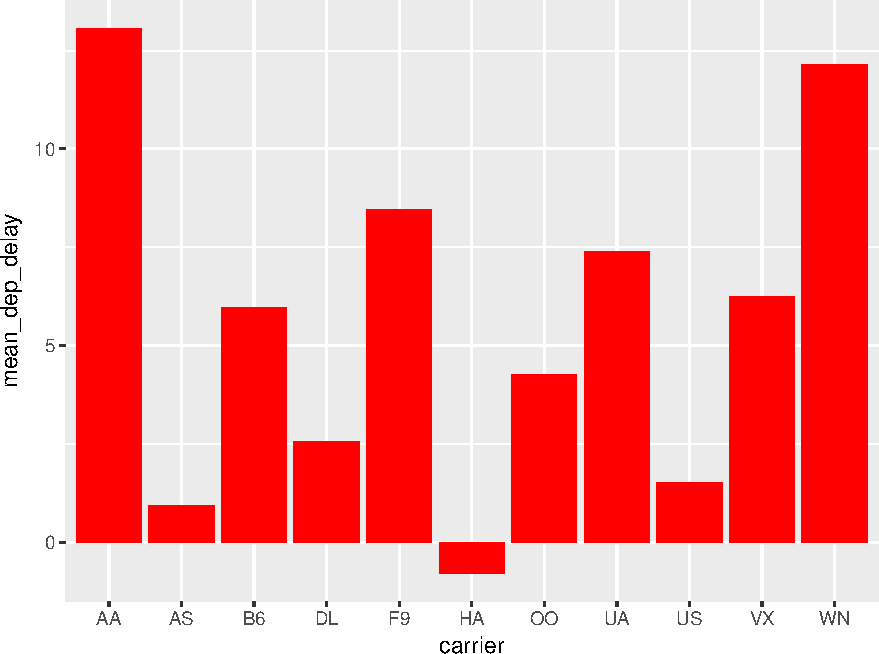
\includegraphics{thesis_files/figure-latex/delaysboxplot-1.pdf}
\caption{\label{fig:delaysboxplot}Mean Delays by Airline}
\end{figure}
Here is a reference to this image: Figure \ref{fig:delaysboxplot}.

A table linking these carrier codes to airline names is available at
\url{https://github.com/ismayc/pnwflights14/blob/master/data/airlines.csv}.

\clearpage

Next, we will explore the use of the \texttt{out.extra} chunk option,
which can be used to shrink or expand an image loaded from a file by
specifying \texttt{"scale=\ "}. Here we use the mathematical graph
stored in the ``subdivision.pdf'' file.
\begin{figure}
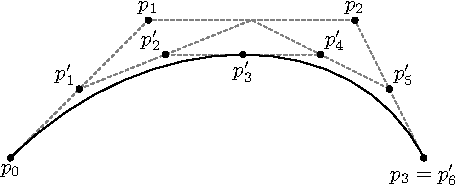
\includegraphics[scale=0.75]{figure/subdivision} \caption{Subdiv. graph}\label{fig:subd}
\end{figure}
Here is a reference to this image: Figure \ref{fig:subd}. Note that
\texttt{echo=FALSE} is specified so that the \textbf{R} code is hidden
in the document.

\textbf{More Figure Stuff}

Lastly, we will explore how to rotate and enlarge figures using the
\texttt{out.extra} chunk option. (Currently this only works in the PDF
version of the book.)
\begin{figure}
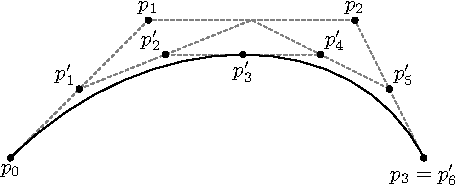
\includegraphics[angle=180, scale=1.1]{figure/subdivision} \caption{A Larger Figure, Flipped Upside Down}\label{fig:subd2}
\end{figure}
As another example, here is a reference: Figure \ref{fig:subd2}.

\section{Footnotes and Endnotes}\label{footnotes-and-endnotes}

You might want to footnote something.\footnote{footnote text} The
footnote will be in a smaller font and placed appropriately. Endnotes
work in much the same way. More information can be found about both on
the CUS site or feel free to reach out to
\href{mailto:data@reed.edu}{\nolinkurl{data@reed.edu}}.

\section{Bibliographies}\label{bibliographies}

Of course you will need to cite things, and you will probably accumulate
an armful of sources. There are a variety of tools available for
creating a bibliography database (stored with the .bib extension). In
addition to BibTeX suggested below, you may want to consider using the
free and easy-to-use tool called Zotero. The Reed librarians have
created Zotero documentation at
\url{http://libguides.reed.edu/citation/zotero}. In addition, a tutorial
is available from Middlebury College at
\url{http://sites.middlebury.edu/zoteromiddlebury/}.

\emph{R Markdown} uses \emph{pandoc} (\url{http://pandoc.org/}) to build
its bibliographies. One nice caveat of this is that you won't have to do
a second compile to load in references as standard LaTeX requires. To
cite references in your thesis (after creating your bibliography
database), place the reference name inside square brackets and precede
it by the ``at'' symbol. For example, here's a reference to a book about
worrying: (Molina \& Borkovec, 1994). This \texttt{Molina1994} entry
appears in a file called \texttt{thesis.bib} in the \texttt{bib} folder.
This bibliography database file was created by a program called BibTeX.
You can call this file something else if you like (look at the YAML
header in the main .Rmd file) and, by default, is to placed in the
\texttt{bib} folder.

For more information about BibTeX and bibliographies, see our CUS site
(\url{http://web.reed.edu/cis/help/latex/index.html})\footnote{Reed~College
  (2007)}. There are three pages on this topic: \emph{bibtex} (which
talks about using BibTeX, at
\url{http://web.reed.edu/cis/help/latex/bibtex.html}),
\emph{bibtexstyles} (about how to find and use the bibliography style
that best suits your needs, at
\url{http://web.reed.edu/cis/help/latex/bibtexstyles.html}) and
\emph{bibman} (which covers how to make and maintain a bibliography by
hand, without BibTeX, at
\url{http://web.reed.edu/cis/help/latex/bibman.html}). The last page
will not be useful unless you have only a few sources.

If you look at the YAML header at the top of the main .Rmd file you can
see that we can specify the style of the bibliography by referencing the
appropriate csl file. You can download a variety of different style
files at \url{https://www.zotero.org/styles}. Make sure to download the
file into the csl folder.

\textbf{Tips for Bibliographies}
\begin{itemize}
\tightlist
\item
  Like with thesis formatting, the sooner you start compiling your
  bibliography for something as large as thesis, the better. Typing in
  source after source is mind-numbing enough; do you really want to do
  it for hours on end in late April? Think of it as procrastination.
\item
  The cite key (a citation's label) needs to be unique from the other
  entries.
\item
  When you have more than one author or editor, you need to separate
  each author's name by the word ``and'' e.g.
  \texttt{Author\ =\ \{Noble,\ Sam\ and\ Youngberg,\ Jessica\},}.
\item
  Bibliographies made using BibTeX (whether manually or using a manager)
  accept LaTeX markup, so you can italicize and add symbols as
  necessary.
\item
  To force capitalization in an article title or where all lowercase is
  generally used, bracket the capital letter in curly braces.
\item
  You can add a Reed Thesis citation\footnote{Noble (2002)} option. The
  best way to do this is to use the phdthesis type of citation, and use
  the optional ``type'' field to enter ``Reed thesis'' or
  ``Undergraduate thesis.''
\end{itemize}
\section{Anything else?}\label{anything-else}

If you'd like to see examples of other things in this template, please
contact the Data @ Reed team (email
\href{mailto:data@reed.edu}{\nolinkurl{data@reed.edu}}) with your
suggestions. We love to see people using \emph{R Markdown} for their
theses, and are happy to help.

\chapter*{Conclusion}\label{conclusion}
\addcontentsline{toc}{chapter}{Conclusion}

If we don't want Conclusion to have a chapter number next to it, we can
add the \texttt{\{-\}} attribute.

\textbf{More info}

And here's some other random info: the first paragraph after a chapter
title or section head \emph{shouldn't be} indented, because indents are
to tell the reader that you're starting a new paragraph. Since that's
obvious after a chapter or section title, proper typesetting doesn't add
an indent there.

\appendix

\chapter{The First Appendix}\label{the-first-appendix}

This first appendix includes all of the R chunks of code that were
hidden throughout the document (using the \texttt{include\ =\ FALSE}
chunk tag) to help with readibility and/or setup.

\textbf{In the main Rmd file}

\textbf{In Chapter \ref{ref-labels}:}
\begin{Shaded}
\begin{Highlighting}[]
\CommentTok{# This chunk ensures that the thesisdown package is}
\CommentTok{# installed and loaded. This thesisdown package includes}
\CommentTok{# the template files for the thesis and also two functions}
\CommentTok{# used for labeling and referencing}
\NormalTok{if(!}\KeywordTok{require}\NormalTok{(devtools))}
  \KeywordTok{install.packages}\NormalTok{(}\StringTok{"devtools"}\NormalTok{, }\DataTypeTok{repos =} \StringTok{"http://cran.rstudio.com"}\NormalTok{)}
\NormalTok{if(!}\KeywordTok{require}\NormalTok{(dplyr))}
    \KeywordTok{install.packages}\NormalTok{(}\StringTok{"dplyr"}\NormalTok{, }\DataTypeTok{repos =} \StringTok{"http://cran.rstudio.com"}\NormalTok{)}
\NormalTok{if(!}\KeywordTok{require}\NormalTok{(ggplot2))}
    \KeywordTok{install.packages}\NormalTok{(}\StringTok{"ggplot2"}\NormalTok{, }\DataTypeTok{repos =} \StringTok{"http://cran.rstudio.com"}\NormalTok{)}
\NormalTok{if(!}\KeywordTok{require}\NormalTok{(ggplot2))}
    \KeywordTok{install.packages}\NormalTok{(}\StringTok{"bookdown"}\NormalTok{, }\DataTypeTok{repos =} \StringTok{"http://cran.rstudio.com"}\NormalTok{)}
\NormalTok{if(!}\KeywordTok{require}\NormalTok{(thesisdown))\{}
  \KeywordTok{library}\NormalTok{(devtools)}
  \NormalTok{devtools::}\KeywordTok{install_github}\NormalTok{(}\StringTok{"ismayc/thesisdown"}\NormalTok{)}
  \NormalTok{\}}
\KeywordTok{library}\NormalTok{(thesisdown)}
\NormalTok{flights <-}\StringTok{ }\KeywordTok{read.csv}\NormalTok{(}\StringTok{"data/flights.csv"}\NormalTok{)}
\end{Highlighting}
\end{Shaded}
\chapter{The Second Appendix, for
Fun}\label{the-second-appendix-for-fun}

\backmatter

\chapter*{References}\label{references}
\addcontentsline{toc}{chapter}{References}

\markboth{References}{References}

\noindent

\setlength{\parindent}{-0.20in} \setlength{\leftskip}{0.20in}
\setlength{\parskip}{8pt}

\hypertarget{refs}{}
\hypertarget{ref-amadeo2017}{}
Amadeo, K. (2017, april). Stock market crash of 2008. \emph{The
Balance}. Retrieved from
\url{https://www.thebalance.com/stock-market-crash-of-2008-3305535}

\hypertarget{ref-angel2000}{}
Angel, E. (2000). \emph{Interactive computer graphics : A top-down
approach with opengl}. Boston, MA: Addison Wesley Longman.

\hypertarget{ref-angel2001}{}
Angel, E. (2001a). \emph{Batch-file computer graphics : A bottom-up
approach with quicktime}. Boston, MA: Wesley Addison Longman.

\hypertarget{ref-angel2002a}{}
Angel, E. (2001b). \emph{Test second book by angel}. Boston, MA: Wesley
Addison Longman.

\hypertarget{ref-baker2011}{}
Baker, M., Bradley, B., \& Wurgler, J. (2011). Benchmarks as limits to
arbitrage: Understanding the low-volatility anomaly. \emph{Financial
Analysts Journal}, \emph{67}(1), 40--54.

\hypertarget{ref-berger2017}{}
Berger, R. (2017, May). Amazon's 49,000. \emph{Forbes}. Forbes Magazine.
Retrieved from
\url{https://www.forbes.com/sites/robertberger/2017/05/20/amazons-49000-return-a-test-for-value-investors/\#7b8efe2049cf)}

\hypertarget{ref-blackrock2017}{}
BlackRock. (2017, September). IShares edge msci min vol usa etf
\textbar{} usmv. Retrieved from
\url{https://www.ishares.com/us/products/239695/ishares-msci-usa-minimum-volatility-etf}

\hypertarget{ref-boyer2009}{}
Boyer, B., Mitton, T., \& Vorkink, K. (2009). Expected idiosyncratic
skewness. \emph{The Review of Financial Studies}, \emph{23}(1),
169--202.

\hypertarget{ref-brennan1989}{}
Brennan, M. J. (1989). Capital asset pricing model. In \emph{Finance}
(pp. 91--102). Springer.

\hypertarget{ref-fama1992}{}
Fama, E. F., \& French, K. R. (1992). The cross-section of expected
stock returns. \emph{The Journal of Finance}, \emph{47}(2), 427--465.

\hypertarget{ref-fischhoff1977}{}
Fischhoff, B., Slovic, P., \& Lichtenstein, S. (1977). Knowing with
certainty: The appropriateness of extreme confidence. \emph{Journal of
Experimental Psychology: Human Perception and Performance}, \emph{3}(4),
552.

\hypertarget{ref-fontinelle2009}{}
Fontinelle, E. (2009, October). ETF tracking errors: Protect your
returns. Retrieved from
\url{http://www.investopedia.com/articles/exchangetradedfunds/09/tracking-error-etf-funds.asp}

\hypertarget{ref-goodwin1998}{}
Goodwin, T. H. (1998). The information ratio. \emph{Financial Analysts
Journal}, \emph{54}(4), 34--43.

\hypertarget{ref-graham1965}{}
Graham, B. (1965). \emph{The intelligent investor: A book of practical
counsel}. Prabhat Prakashan.

\hypertarget{ref-haugen1975}{}
Haugen, R. A., \& Heins, J. A. (1975). Risk and the rate of return on
financial assets: Some old wine in new bottles. \emph{Journal of
Financial and Quantitative Analysis}, \emph{10}(5), 775--784.

\hypertarget{ref-hayes2017}{}
Hayes, A. (2017, October). Exchange-traded fund (etf). Retrieved from
\url{http://www.investopedia.com/terms/e/etf.asp}

\hypertarget{ref-history2010}{}
History. (2010). Stock market crash of 1929. \emph{History.com}. A\&E
Television Networks. Retrieved from
\url{http://www.history.com/topics/1929-stock-market-crash}

\hypertarget{ref-investopedia2015}{}
Investopedia. (2015, April). What are some common measures of risk used
in risk management? \emph{Investopedia}. Retrieved from
\url{http://www.investopedia.com/ask/answers/041415/what-are-some-common-measures-risk-used-risk-management.asp}

\hypertarget{ref-investopedia2017}{}
Investopedia. (2017, February). Two and twenty. \emph{Investopedia}.
Retrieved from
\url{http://www.investopedia.com/terms/t/two_and_twenty.asp}

\hypertarget{ref-jensen1972}{}
Jensen, M. C., Black, F., \& Scholes, M. S. (1972). The capital asset
pricing model: Some empirical tests.

\hypertarget{ref-karceski2002}{}
Karceski, J. (2002). Returns-chasing behavior, mutual funds, and beta's
death. \emph{Journal of Financial and Quantitative Analysis},
\emph{37}(4), 559--594.

\hypertarget{ref-macdonald2009}{}
MacDonald, L. (2009, october). How traders are front-running etfs.
Retrieved from
\url{https://seekingalpha.com/article/165877-how-traders-are-front-running-etfs}

\hypertarget{ref-Molina1994}{}
Molina, S. T., \& Borkovec, T. D. (1994). The Penn State worry
questionnaire: Psychometric properties and associated characteristics.
In G. C. L. Davey \& F. Tallis (Eds.), \emph{Worrying: Perspectives on
theory, assessment and treatment} (pp. 265--283). New York: Wiley.

\hypertarget{ref-msci2013}{}
MSCI. (2013, September). Barra open optimizer. Retrieved from
\url{https://www.msci.com/documents/10199/242721/Barra_Optimizer.pdf/5acf4515-dbd8-4d0c-8acc-ca70b7b68f69}

\hypertarget{ref-mullins1982}{}
Mullins, D. W. (1982). Does the capital asset pricing model work.
\emph{Harvard Business Review}, \emph{60}(1), 105--113.

\hypertarget{ref-noble2002}{}
Noble, S. G. (2002). \emph{Turning images into simple line-art}
(Undergraduate thesis). Reed College.

\hypertarget{ref-ontario2017}{}
Ontario, S. C. (2017, May). Types of investment risk \textbar{}
understanding risk. Retrieved from
\url{https://www.getsmarteraboutmoney.ca/invest/investing-basics/understanding-risk/types-of-investment-risk/}

\hypertarget{ref-pettengill1995}{}
Pettengill, G. N., Sundaram, S., \& Mathur, I. (1995). The conditional
relation between beta and returns. \emph{Journal of Financial and
Quantitative Analysis}, \emph{30}(1), 101--116.

\hypertarget{ref-reedweb2007}{}
Reed~College. (2007, march). LaTeX your document. Retrieved from
\url{http://web.reed.edu/cis/help/LaTeX/index.html}

\hypertarget{ref-sensoy2009}{}
Sensoy, B. A. (2009). Performance evaluation and self-designated
benchmark indexes in the mutual fund industry. \emph{Journal of
Financial Economics}, \emph{92}(1), 25--39.

\hypertarget{ref-van2016}{}
Vliet, P. V., \& Koning, J. de. (2016). \emph{High returns from low
risk: A remarkable stock market paradox}. John Wiley \& Sons.

\hypertarget{ref-wynne2016}{}
Wynne, B. (2016, april). Understanding the iShares msci usa minimum
volatility etf. Retrieved from
\url{https://seekingalpha.com/article/3964639-understanding-ishares-msci-usa-minimum-volatility-etf}


% Index?

\end{document}
